% This is the default LaTeX template (default-1.17.0.2.tex) from the RMarkdown package, from:
% https://github.com/rstudio/rmarkdown/blob/master/inst/rmd/latex/default-1.17.0.2.tex
%
% New additions to the template are marked with "LCR"

%\documentclass[12pt,english,]{book} %LCR
 % if not, force the oneside and a4paper options, which seem to be the only reasonable defaults
\documentclass[12pt,a4paper,oneside,]{book} %LCR


% Looad graphicx for images
\usepackage{graphicx}

% Load Linux Libertine font package
\usepackage{libertine}

% Set the main font family to Libertine
\renewcommand{\familydefault}{\sfdefault}

% Set the sans-serif font family to Libertine (optional)
\renewcommand{\sfdefault}{lmss}

% Set the monospace font family to Libertine (optional)
\renewcommand{\ttdefault}{lmtt}


\usepackage{amssymb,amsmath}
\usepackage{ifxetex,ifluatex}
\usepackage{fixltx2e} % provides \textsubscript
\ifnum 0\ifxetex 1\fi\ifluatex 1\fi=0 % if pdftex
  \usepackage[T1]{fontenc}
  \usepackage[utf8]{inputenc}
\else % if luatex or xelatex
  \ifxetex
    \usepackage{mathspec}
  \else
    \usepackage{fontspec}
  \fi
  \defaultfontfeatures{Ligatures=TeX,Scale=MatchLowercase}
\fi
% use upquote if available, for straight quotes in verbatim environments
\IfFileExists{upquote.sty}{\usepackage{upquote}}{}
% use microtype if available
\IfFileExists{microtype.sty}{%
\usepackage{microtype}
\UseMicrotypeSet[protrusion]{basicmath} % disable protrusion for tt fonts
}{}

 %LCR
\usepackage{hyperref}
\hypersetup{unicode=true,
            pdftitle={PhD Evaluation: 9-month Report},
            pdfauthor={Aamir Sohail},
            pdfborder={0 0 0},
            breaklinks=true}
\urlstyle{same}  % don't use monospace font for urls
\ifLuaTeX
\usepackage[bidi=basic]{babel}
\else
\usepackage[bidi=default]{babel}
\fi
\babelprovide[main,import]{english}
% get rid of language-specific shorthands (see #6817):
\let\LanguageShortHands\languageshorthands
\def\languageshorthands#1{}
\usepackage{longtable,booktabs}
% Make links footnotes instead of hotlinks:
\renewcommand{\href}[2]{#2\footnote{\url{#1}}}
\setlength{\emergencystretch}{3em}  % prevent overfull lines
\providecommand{\tightlist}{%
  \setlength{\itemsep}{0pt}\setlength{\parskip}{0pt}}
\setcounter{secnumdepth}{5}
% Redefines (sub)paragraphs to behave more like sections
\ifx\paragraph\undefined\else
\let\oldparagraph\paragraph
\renewcommand{\paragraph}[1]{\oldparagraph{#1}\mbox{}}
\fi
\ifx\subparagraph\undefined\else
\let\oldsubparagraph\subparagraph
\renewcommand{\subparagraph}[1]{\oldsubparagraph{#1}\mbox{}}
\fi

% LCR: fix for new required cslreferences environment in pandoc
% from https://github.com/rstudio/rticles/blob/81bb6816a42797f66fbbc6d7c92ffd8216783ed3/inst/rmarkdown/templates/elsevier/resources/template.tex#L146-L177

%%% Use protect on footnotes to avoid problems with footnotes in titles
\let\rmarkdownfootnote\footnote%
\def\footnote{\protect\rmarkdownfootnote}

%%% This fixes a TexLive 2019 change that broke pandoc template. Will also be fixed in pandoc 2.8 %LCR
% https://github.com/jgm/pandoc/issues/5801
\renewcommand{\linethickness}{0.05em}

%%%%%%%%%%%%% BEGIN DOCUMENT %%%%%%%%%%%%%
\begin{document}

%% Page I: the half-title / "Franse pagina" %LCR
\frontmatter
\thispagestyle{empty}
\def\drop{.1\textheight}

\vspace*{\drop}
\begin{center}
\Huge \textsc{PhD Evaluation: 9-month Report}
\end{center}

%% Page III: `Title page' 
\clearpage
\thispagestyle{empty}
\vspace*{\drop}
\begin{center}
    
\includegraphics[width=0.3\textwidth]{figures/birmingham.png} % Adjust the width as desired
\end{center}
\vspace{\baselineskip}

\begin{center}
\Huge\textbf{PhD Evaluation: 9-month Report}\par
\vfill % this space will be whatever is left on the page
{\huge Aamir Sohail}\par
\vspace{1em}
\linespread{1.3}{\normalsize Centre for Human Brain Health\\
University of Birmingham\\ }\par %
\vspace{\baselineskip}
{\normalsize under the supervision of:}\par
{\Large Dr. Lei Zhang\\
Professor Patricia L. Lockwood}\par
\vspace{\baselineskip}
{\small Word Count: 4992}
\end{center}

%%%%%%%%%%%%%%%%%%


{
\setcounter{tocdepth}{1}
\tableofcontents
}
\mainmatter
\chapter{Introduction}\label{introduction}

\emph{This report summarises the three studies that I plan to run during my PhD, which aims to uncover the neurocomputational mechanisms of social learning and how this is altered in psychopathology}.

\emph{I firstly provide a detailed account of my initial behavioural study examining transdiagnostic influences on observational and experiential learning by performing a review of the relevant literature, before discussing the methods and hypothesised results. Following this, two neuroimaging studies where I aim to uncover the neurocomputational mechanisms underlying social learning in social anxiety, and its treatment using smartphone-delivered CBT, will be briefly outlined}.

\emph{Together, this research will provide a formal account of social learning grounded in computational neuroscience, informing novel methods of psychiatric treatment}.

\begin{center}\rule{0.5\linewidth}{0.5pt}\end{center}

\chapter{Uncovering transdiagnostic influences on experiential and observational learning: a study plan}\label{uncovering-transdiagnostic-influences-on-experiential-and-observational-learning-a-study-plan}

\chaptermark{}

\section{Introduction}\label{introduction-1}

Decision-making in humans is guided by learning, both from personal experience, and the actions and choices of others (Lee et al., 2012; O'Doherty et al., 2017; Sutton \& Barto, 2018). The former reflects experiential learning (EL) (O'Doherty et al., 2004), where actions that were previously rewarded are more likely to be re-selected, while actions previously punished are more likely to be avoided. Conversely, observational learning (OL) (Joiner et al., 2017) is vicarious, by which agents are able to determine the rewarding or punishing outcomes associated with specific actions without the need to personally engage in exploratory or risky behaviour (Dunne \& O'Doherty, 2013). To this end, agents learn to imitate or develop a causal understanding of others' successful actions (Cushman, 2024; Suzuki \& O'Doherty, 2020), by employing several strategies including the capacity to learn from the rewards experienced by others, and from inferring their goals/intentions (Charpentier \& O'Doherty, 2018; O'Doherty et al., 2021).

In certain social environments, humans may integrate both OL and EL in the decision-making process (Charpentier et al., 2023; Pärnamets \& Olsson, 2020; Zhang \& Gläscher, 2020), by tracking signals associated with direct experience and vicarious valuation with a combined reward/social prediction error (Zhang \& Gläscher, 2020). However, there is considerable heterogeneity across individuals who may also switch between EL and OL according to the reliability of each strategy (O'Doherty et al., 2021), or evoke a single strategy of EL-only or OL-only (Charpentier et al., 2023). Ultimately, OL and EL, either collectively, sequentially, or separately, are integral processes when making informed social decisions in complex environments.

Computational frameworks also provide a formal account of behavioural changes observed in mental health disorders (Huys et al., 2016, 2021), where model parameters can be objectively compared across cohorts. Recent literature has shown learning biases across a range of psychopathologies, including difficulties with learning from uncertainty (Aylward et al., 2019; Browning et al., 2015) and punishment (Pike \& Robinson, 2022) among those with mood and anxiety disorders, whilst several studies have demonstrated an association between anhedonia, the core symptom of depression, with reduced learning from rewarding outcomes (Admon \& Pizzagalli, 2015; Eshel \& Roiser, 2010). Furthermore, individuals with social anxiety demonstrate biased learning from socially-specific information (Beltzer et al., 2019; Piray et al., 2019), including positive and negative social feedback (Button et al., 2012; Koban et al., 2017, 2023; Zabag et al., 2022, 2023), and are more accurate at learning to avoid social punishment (Abraham \& Hermann, 2015; Voegler et al., 2019). These learning biases lead to the behavioural symptoms observed in social anxiety, including the maintenance of a negative self-view and low self-esteem (Koban et al., 2017), perception of low social rank (Gilboa-Schechtman et al., 2017) and the continued avoidance of social situations (Peterburs et al., 2022).

However, conventional RL paradigms used to assess social learning do not accurately represent complex social environments, where agents may integrate multiple learning strategies in the decision-making process. To this end, neuroeconomic games present an ecologically valid approach for assessing social behaviour by replicating real-world social interactions in a controlled setting (Glimcher, 2014; Loewenstein et al., 2008), a methodology highly recommended for use in behavioural and psychiatric studies due to its wide applicability (Hasler, 2012; Kishida et al., 2010; Montague, 2018; Robson et al., 2020). In such games, individuals with social anxiety are more likely to conform to others' behaviour or judgements (Bică et al., 2021; Feng et al., 2018), reflecting an excessive need for social approval (Leary et al., 1988). Similarly, clinically depressed individuals are more susceptible to informational social influence (Hofheinz et al., 2017), influenced by self-esteem, a negative predictor of social anxiety (Fatima \& Ghayas, 2017; Seema \& Kumar, 2017). Individuals with low trait self-esteem are also more heavily influenced by others when making social decisions (Lee \& Chung, 2022), suggesting that socially anxious individuals demonstrate a bias towards observational learning.

A major goal of psychological research revolves around associating changes in task performance with behavioural traits or measurements. Yet, measures of psychopathology are conventionally reduced to a single dimension or score, despite high-levels of heterogeneity observed among psychiatric disorders (Feczko et al., 2019), including social anxiety disorder (SAD) (Spokas \& Cardaciotto, 2014) and depression (Fried, 2017), reflecting a complex behavioural profile not captured by a single dimension or questionnaire. A transdiagnostic approach to psychopathology (Gillan et al., 2016; Robbins et al., 2012) conversely favours a continuous definition of mental illness, present among normal variations in psychopathology in the general population. By employing data-driven dimensionality reduction on questionnaire batteries assessing a wide-berth of psychopathology, latent factors of mental health can be extracted that more accurately map onto candidate learning processes than any individual questionnaire score (Gillan \& Seow, 2020). Computational factor modeling (CFM) (Wise et al., 2023) further combines a transdiagnostic approach with theory-driven computational modeling of behaviour, to infer the computational processes that characterize a given factor. To date, CFM has identified transdiagnostic associations with model-based planning (Gillan et al., 2016), metacognition (Rouault et al., 2018), reward processing (Suzuki et al., 2021) and uncertainty (Norbury et al., 2018), offering an objective formal approach for demonstrating learning biases at the transdiagnostic level.

To date, a single study has applied a transdiagnostic approach to EL and OL, finding that heterogeneity in strategy use is characterized along the two psychiatric symptom dimensions of autistic traits and trait anxiety (Charpentier et al., 2023). Surprisingly, there were no significant influence of the transdiagnostic dimensions of social anxiety or social dysfunction. This may be a consequence of the task design, which only involved observation of a single other simulated agent, differing from complex social environments where agents must learn from multiple others. Furthermore, the study did not measure the behavioural effects of confidence, which influences choice (Campbell-Meiklejohn et al., 2017; De Martino et al., 2013) and is negatively correlated with self-reported depression, social anxiety, and generalized anxiety scores (Rouault et al., 2018). In addition, the questionnaire battery consisting of only four questionnaires excludes certain components of psychopathology, with the latent factor structure unvalidated. A more comprehensive, validated battery may therefore be more suitable for extracting latent factors of psychopathology.

In our planned study, we aim to identify the transdiagnostic symptom dimensions underlying OL and EL by recruiting a large general population sample, tasked with completing a social influence task in groups. We will dissect the specific contributions of OL and EL to the decision-making process through computational modeling, identifying heterogeneity in strategy use across the whole group, and across transdiagnostic factors. By taking an objective, computational approach, we aim to identify candidate learning processes that can be targeted through pharmacological and psychotherapeutic interventions.

\section{Methods}\label{methods}

\subsection{Participants}\label{participants}

Participants will be recruited from the online platform Prolific, with only those between the ages of 18-50, a completion rate of 95\% and with more than 20 completed studies eligible. We aim to recruit 500 participants, similar to previous studies (Hoven et al., 2023; Rouault et al., 2018; Seow \& Gillan, 2020) demonstrating a strong replicability of the original factor loadings reported in a larger sample (Gillan et al., 2016). Given the average exclusion rate of approximately 15\% for online behavioural studies (Chandler et al., 2014) we aim to initially recruit 600 participants. Exclusion criteria will include a history or current diagnosis of neurological/psychiatric disease or current medication. To avoid gender bias, each group will consist of only same-gender participants.

\subsection{Assessments}\label{assessments}

Participants will firstly complete a questionnaire battery (Gillan et al., 2016), reliably assessing a wide berth of psychopathology in a general population sample. Specifically, we will run a reduced sample of 71 questions reliably found to replicate the same 3-factor structure, to increase participant retention (Hopkins et al., 2022). The questionnaire battery will assess obsessive-compulsive disorder (OCD) using the Obsessive-Compulsive Inventory -- Revised (OCI-R) (Foa et al., 2002), depression using the Self-Rating Depression Scale (SDS) (Zung, 1965) trait anxiety using the trait portion of the State-Trait Anxiety Inventory (STAI) (Spielberger, 1970), apathy using the Apathy Evaluation Scale (AES) (Marin et al., 1991), eating disorders using the Eating Attitudes Test (EAT-26) (Garner et al., 1982), impulsivity using the Barratt Impulsivity Scale (BIS-10) (Patton et al., 1995), and social anxiety using the Liebowitz Social Anxiety Scale (LSAS) (Liebowitz, 1987). IQ will also be measured as a co-variate using the Wechsler Adult Intelligence Scale (WAIS) (Wechsler, 2019).

\subsection{Task structure}\label{task-structure}

After completing the questionnaires on Prolific, participants will be invited in groups of five later the same day to complete a social influence task (Zhang \& Gläscher, 2020), a multistage group decision-making paradigm enabling participants to learn directly from their own experience and vicariously from observing others. The task will be implemented using oTree (Chen et al., 2016), an open-source platform with the capacity to real-time multi-player experiments online. The basic experimental setup consists of an experiment written within oTree, a server computer, which can be a cloud server or a local laptop, and subjects' devices with a web browser to access the experiment (Fig 2.1). We selected oTree over alternative platforms including LIONESS Lab (Giamattei et al., 2020) and nodeGame (Balietti, 2017), due to its minimalistic and robust framework, as well as its popularity (\textgreater1900 citations as of May 2024).

\begin{figure}
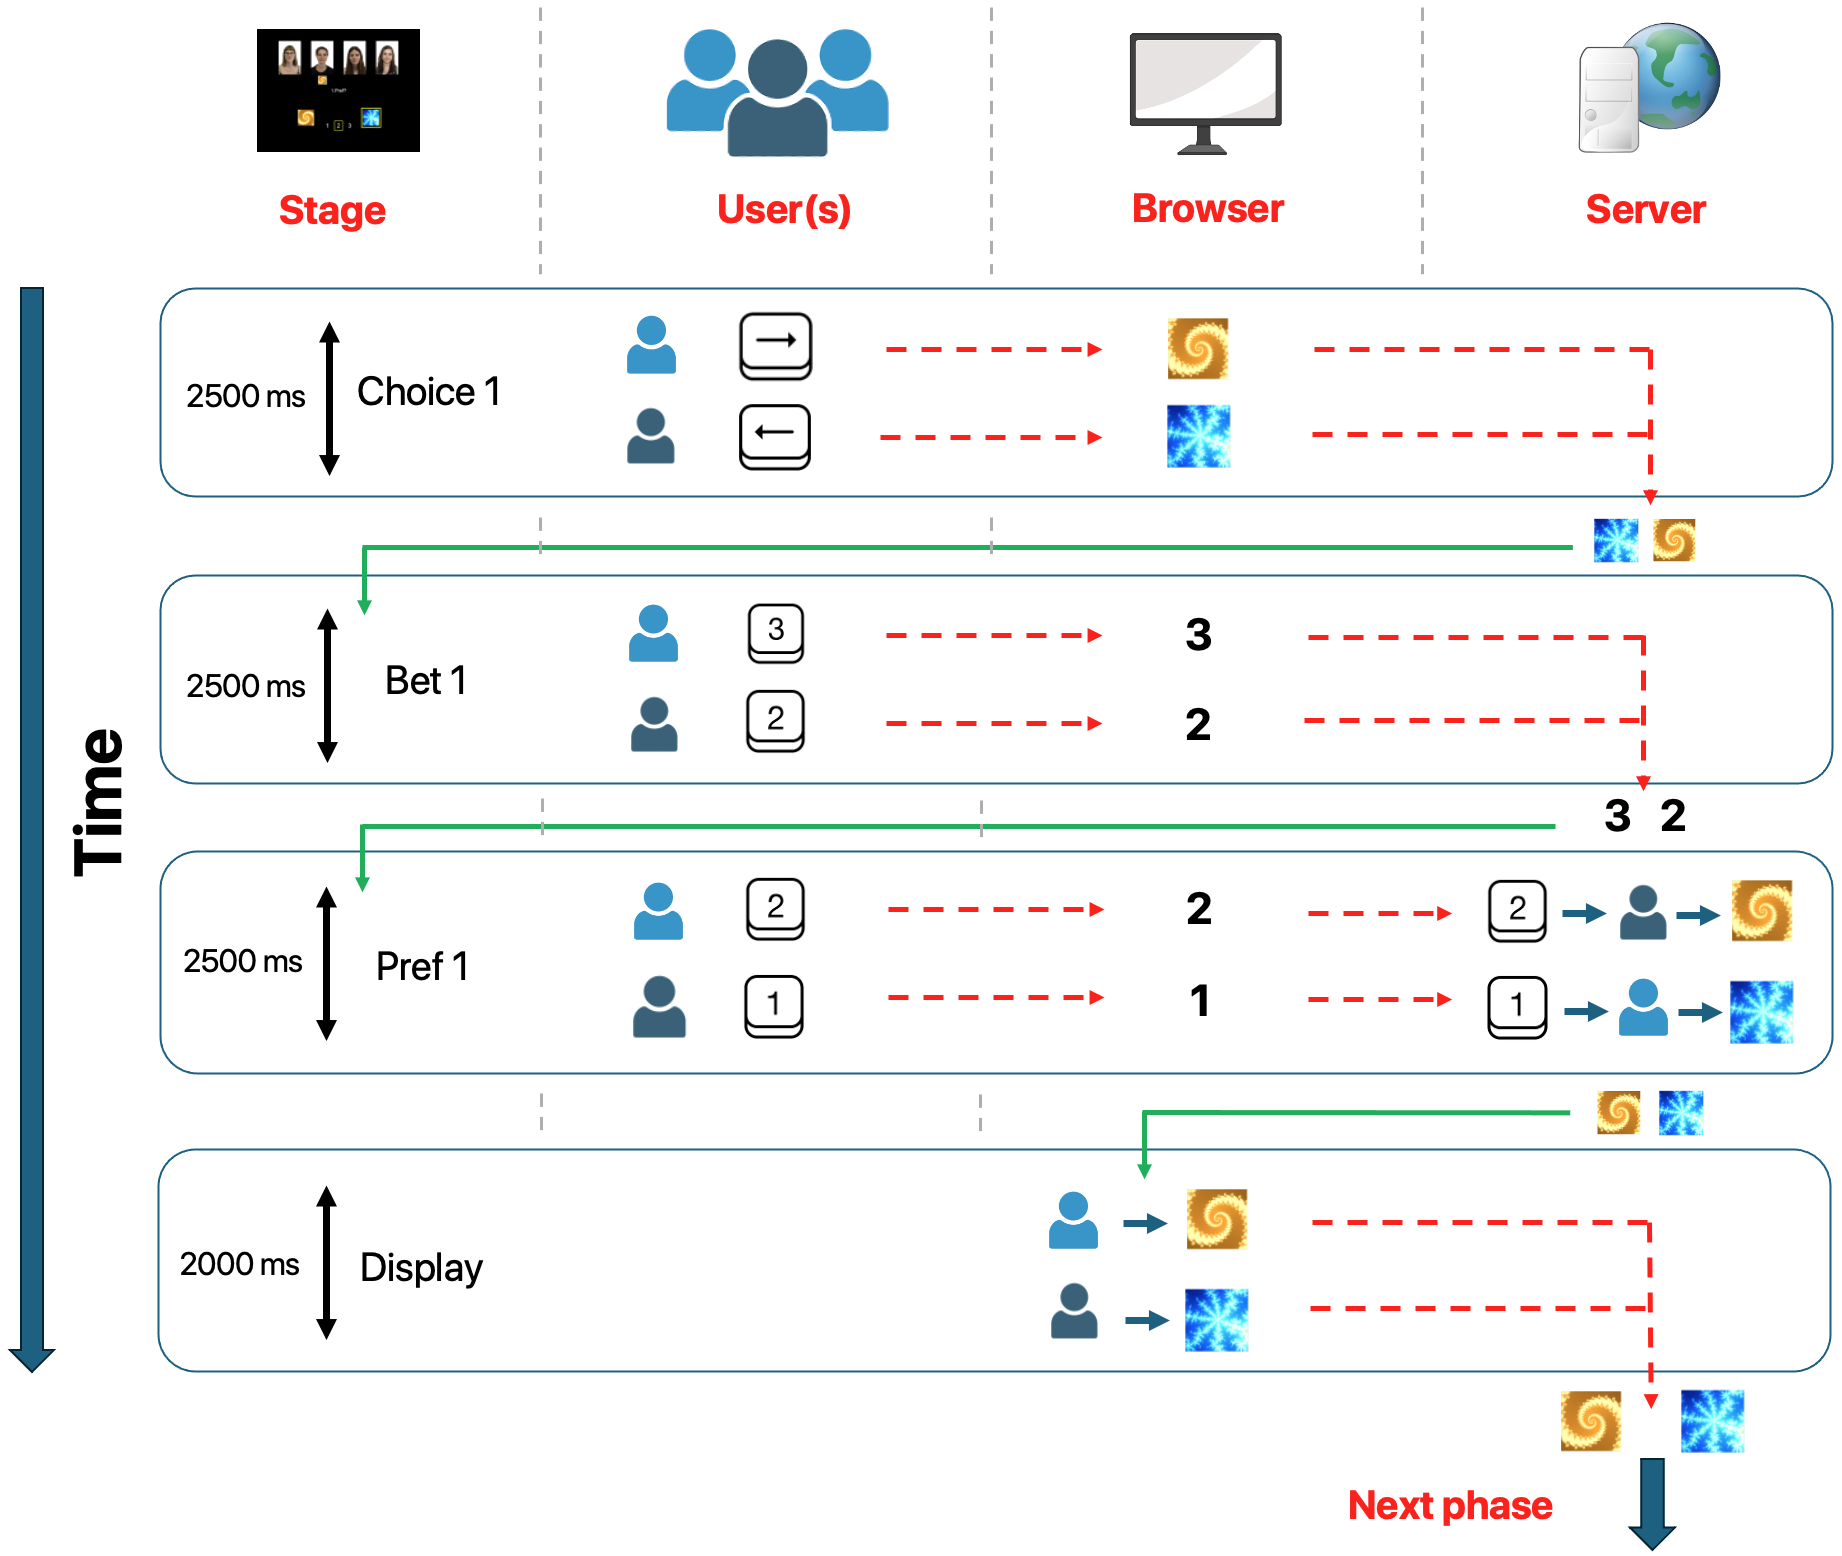
\includegraphics[width=1\linewidth]{figures/otree_flowchart} \caption{{\textbf{The oTree framework for a single page of the social influence task.} When beginning the task, the player firstly enters their initial choice of the two fractals by pressing either the left or right arrow key. At the time of the button press, this response is both logged by the browser locally, and on the server. Subsequently, the end of the Choice 1 phase (determined by the end of a 2500ms interval) triggers the Bet 1 phase, where players must make their bet by pressing either the `1', `2' or `3' button. Players' button presses are similarly logged by the browser and sent to the server at the time of the bet being made. Players are moved to the preference choice phase at the end of the allotted time. In the preference choice phase, players must select another participant within the group whose choice they will uncover. The button press is similarly logged, corresponding to the number assigned to the other players within the group. The server then retrieves the image selected by the player chosen in the choice phase. These images are then displayed, after which players are moved on to the next page consisting of the second choice, second bet and trial feedback. The page structure depicted reflects a simplified version of the actual task.}}\label{fig:figure-1-otree}
\end{figure}



Upon joining a session, participants will be given detailed instructions regarding the task, after which they will individually play a practice session of 10 trials against four computerized opponents. They will then be placed into a waiting room for the other four players to arrive at the same point. The waiting room will include a `live chat' function, both to reduce participant dropout and to demonstrate the legitimacy of the experiment. Once all five players have entered the chat room, after 30 seconds they will be transferred to the main experiment.

Players will then complete the social influence paradigm, a two-alternative forced choice probabilistic reversal-learning task, where each of the two choice options is associated with a particular reward probability (i.e., 70 and 30\%). After a variable length of trials (randomly sampled from a uniform distribution between 8 and 12 trials), the reward contingencies will reverse, such that players needed to readapt to the new reward contingencies to maximize their outcome. The social influence task contains six phases. Firstly, participants will be presented with two choice options using abstract fractals, and asked to make their initial choice, after which participants are asked to indicate how confident they were in their choice, being ``1'' (not confident), ``2'' (reasonably confident), or ``3'' (very confident). Once all participants have provided their Choice 1 and Bet 1, the choices (but not the bets) of the other coplayers will be revealed below their respective avatar. Crucially, instead of seeing all four other choices at the same time, participants can sequentially uncover the decisions of two players in the group. The remaining two choices are displayed automatically afterward. When all four other choices are presented, participants will be able to adjust their choices and their bets, where other coplayers' Choice 2 are also displayed after submitting their adjusted bets. Lastly, the outcome will be determined by the combination of participants' Choice 2 and Bet 2. The social influence paradigm will consist of 100 trials. Following completion of the task, participants will be debriefed regarding the nature of the study, whether they thought they were playing against real or computerized opponents, a potential confound upon choice behaviour in social decision-games (Fig 2.2).

\begin{figure}
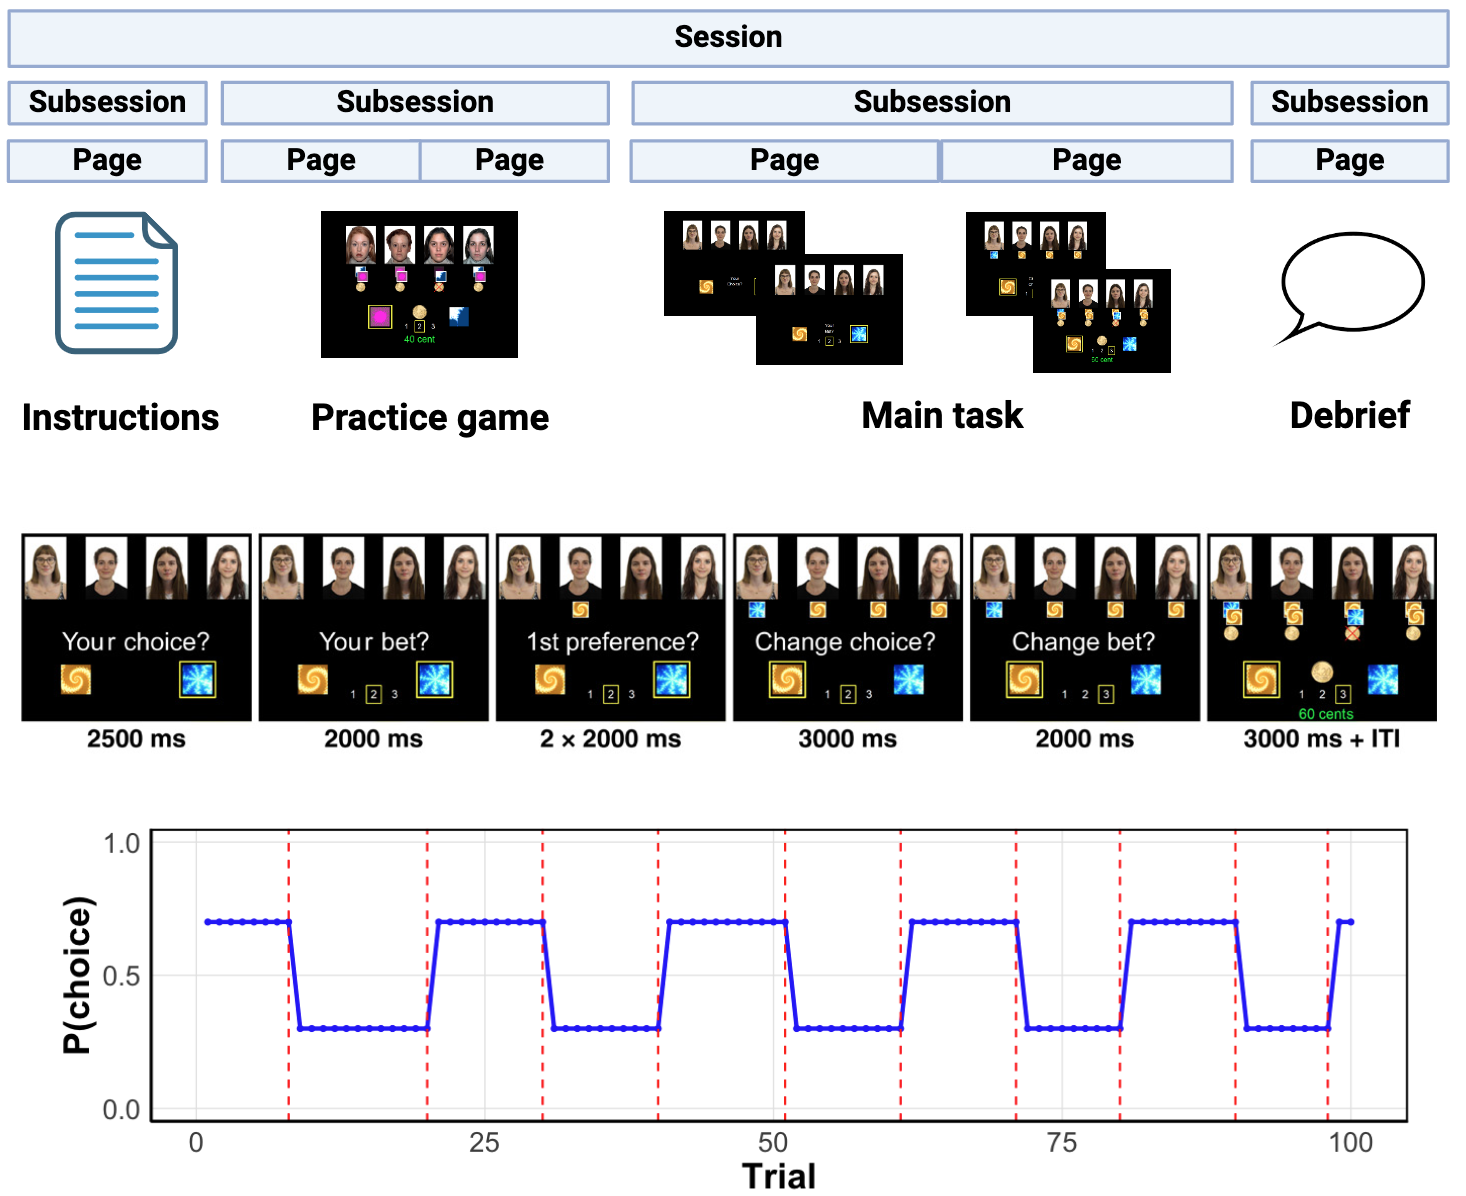
\includegraphics[width=1\linewidth]{figures/otree_experiment} \caption{{\textbf{The general structure of the experiment under the oTree framework.} Each `Session' consists of several `Subsessions' which constitute a distinct component of the experiment. Each `Subsession' itself consists of `Pages' representing each stage of the task. The main social influence task consists of two main pages with page one containing the Choice 1, Bet 1 and Preference phases, whilst page two contains the Choice 2, Bet 2 and trial feedback. Each of the six stages are visually depicted along with the allotted time. Certain components of the figure adapted with permission from (Zhang \& Gläscher, 2020).}}\label{fig:figure-2-otree}
\end{figure}



\section{Planned analyses and results}\label{planned-analyses-and-results}

\subsection{Factor analysis}\label{factor-analysis}

Replicating a popular approach implemented in previous studies (Gillan et al., 2016; Hoven et al., 2023; Rouault et al., 2018; Seow \& Gillan, 2020), we aim to perform our factor analysis with Maximum Likelihood Estimation (MLE) using the Psych package in R, with an oblique rotation. We will subsequently select the number of factors based on Cattell's criterion (Cattell, 1966), using the Cattell-Nelson-Gorsuch test (Gorsuch, 2014). Replicating previous research, we expect a three-factor model `Anxious-Depression', `Compulsive Behaviour and Intrusive Thought' and `Social Withdrawal' to best describe the data structure. Our factor analysis will be validated by running Pearson's correlations between item loadings obtained from the factor analysis in (Hopkins et al., 2022) using the same 71 items (Fig 2.3).

\begin{figure}
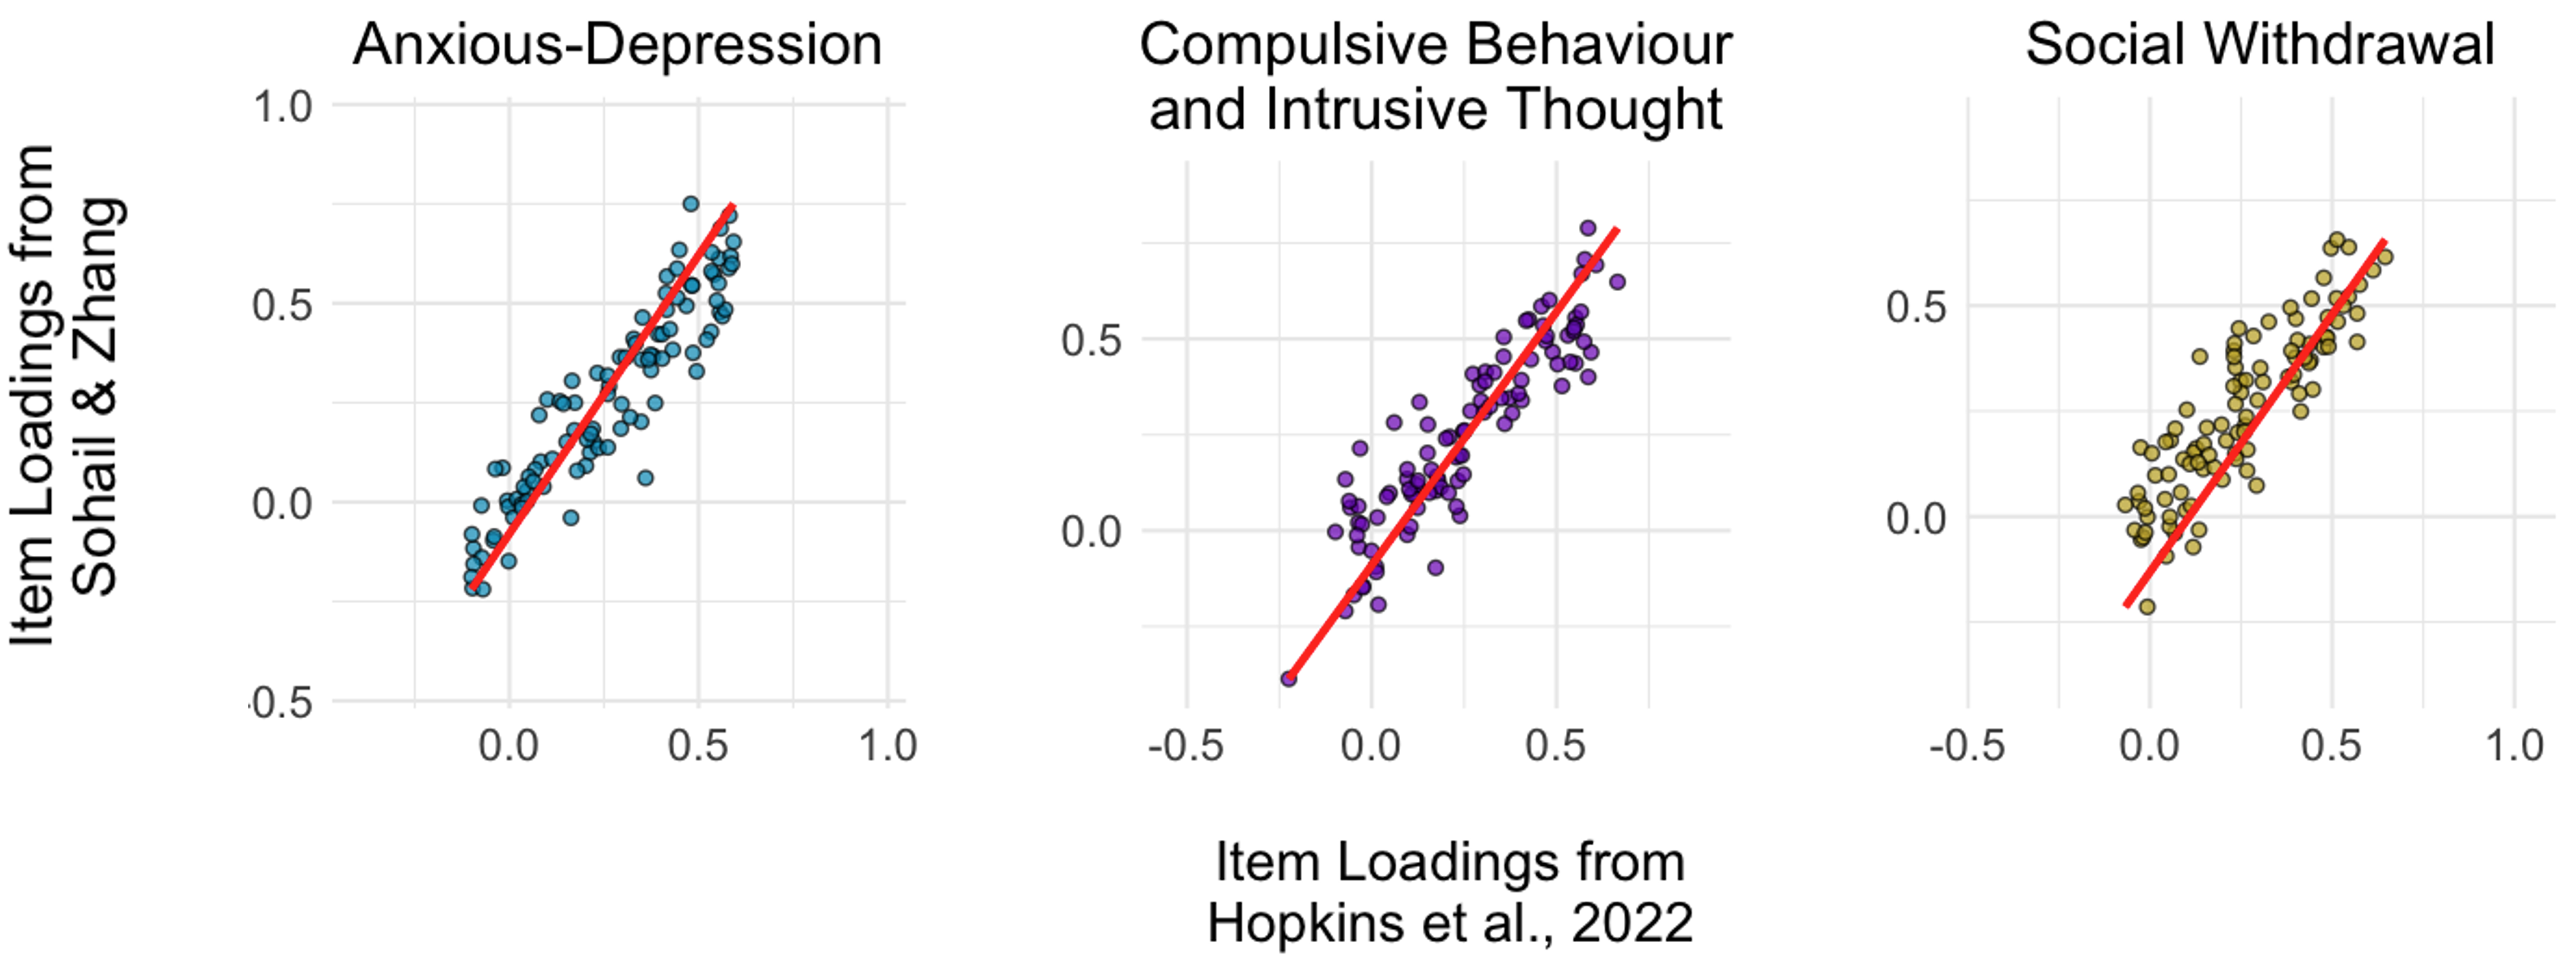
\includegraphics[width=1\linewidth]{figures/factor_correlations} \caption{{\textbf{Predicted correlations between item questionnaire loadings for the study and (Hopkins et al., 2022).}}}\label{fig:figure-3-factor-correlations}
\end{figure}



\subsection{Behavioural analysis}\label{behavioural-analysis}

Across the whole cohort, we look to replicate the behavioural results reported by (Zhang \& Gläscher, 2020), who also ran the same paradigm in a healthy population sample. Namely that:

\begin{enumerate}
\def\labelenumi{\arabic{enumi}.}
\item
  Participants will show an increasing trend to switch their choice toward the group when faced with more dissenting social information, and are more likely to persist when observing agreement with the group.
\item
  Participants will tend to increase their bets as a function of the group consensus when observing confirming opinions but sustain their bets when being contradicted by the group.
\item
  Participants' choice accuracy of the second decision will be significantly higher than that of the first, and participants' second bet will be significantly larger than their first.
\end{enumerate}

To determine the transdiagnostic effects upon these behavioural measures, we plan to run moderation analyses for each factor separately. Reflecting higher levels of social influence on choice through lowered confidence and higher social approval, we expect to see the following associations with both the `Social Withdrawal' and `Anxious-Depression' transdiagnostic factors:

\begin{enumerate}
\def\labelenumi{\arabic{enumi}.}
\item
  An increased tendency to conform to group choices when observing agreement.
\item
  A reduced tendency to increase their bets when observing confirming opinions, and increased tendency to lower their bets when being contradicted.
\item
  Participants' choice accuracy of the second decision will be significantly higher than that of the first, whilst participants' second bet will not significantly differ from the first.
\end{enumerate}

\subsection{Computational modeling}\label{computational-modeling}

To uncover the distinct influence of OL and EL on social decision-making, we will perform trial-by-trial modeling under the hierarchical Bayesian framework using RStan. We will use the same range of non-social and social computational models as a previous study implementing the same paradigm (Zhang \& Gläscher, 2020). These firstly include baseline models which did not consider any social information (category 1: M1a, M1b, and M1c). Instantaneous social influence (i.e., other players' Choice 1, before outcomes were delivered) was then included on top of category 1 models, to construct the first category of social models (category 2: M2a, M2b, and M2c). And finally, social learning parameters were added, reflecting competing hypotheses of value update from observing others (category 3: M3, M4, M5, M6a, and M6b). However, instead of describing a singular `winning' model explaining all participants' data, we aim to implement a heterogeneous approach used to describe different strategies employed across the sample (Charpentier et al., 2023). To this end, we aim to fit the same models to each individual, calculating the winning frequency of each model across all participants (Fig 2.4). Model verification will be performed through a parameter recovery analysis to assure that all parameters can be accurately and selectively identified, and posterior predictive checks which should accurately capture behavioural patterns observed in the data.

\begin{figure}
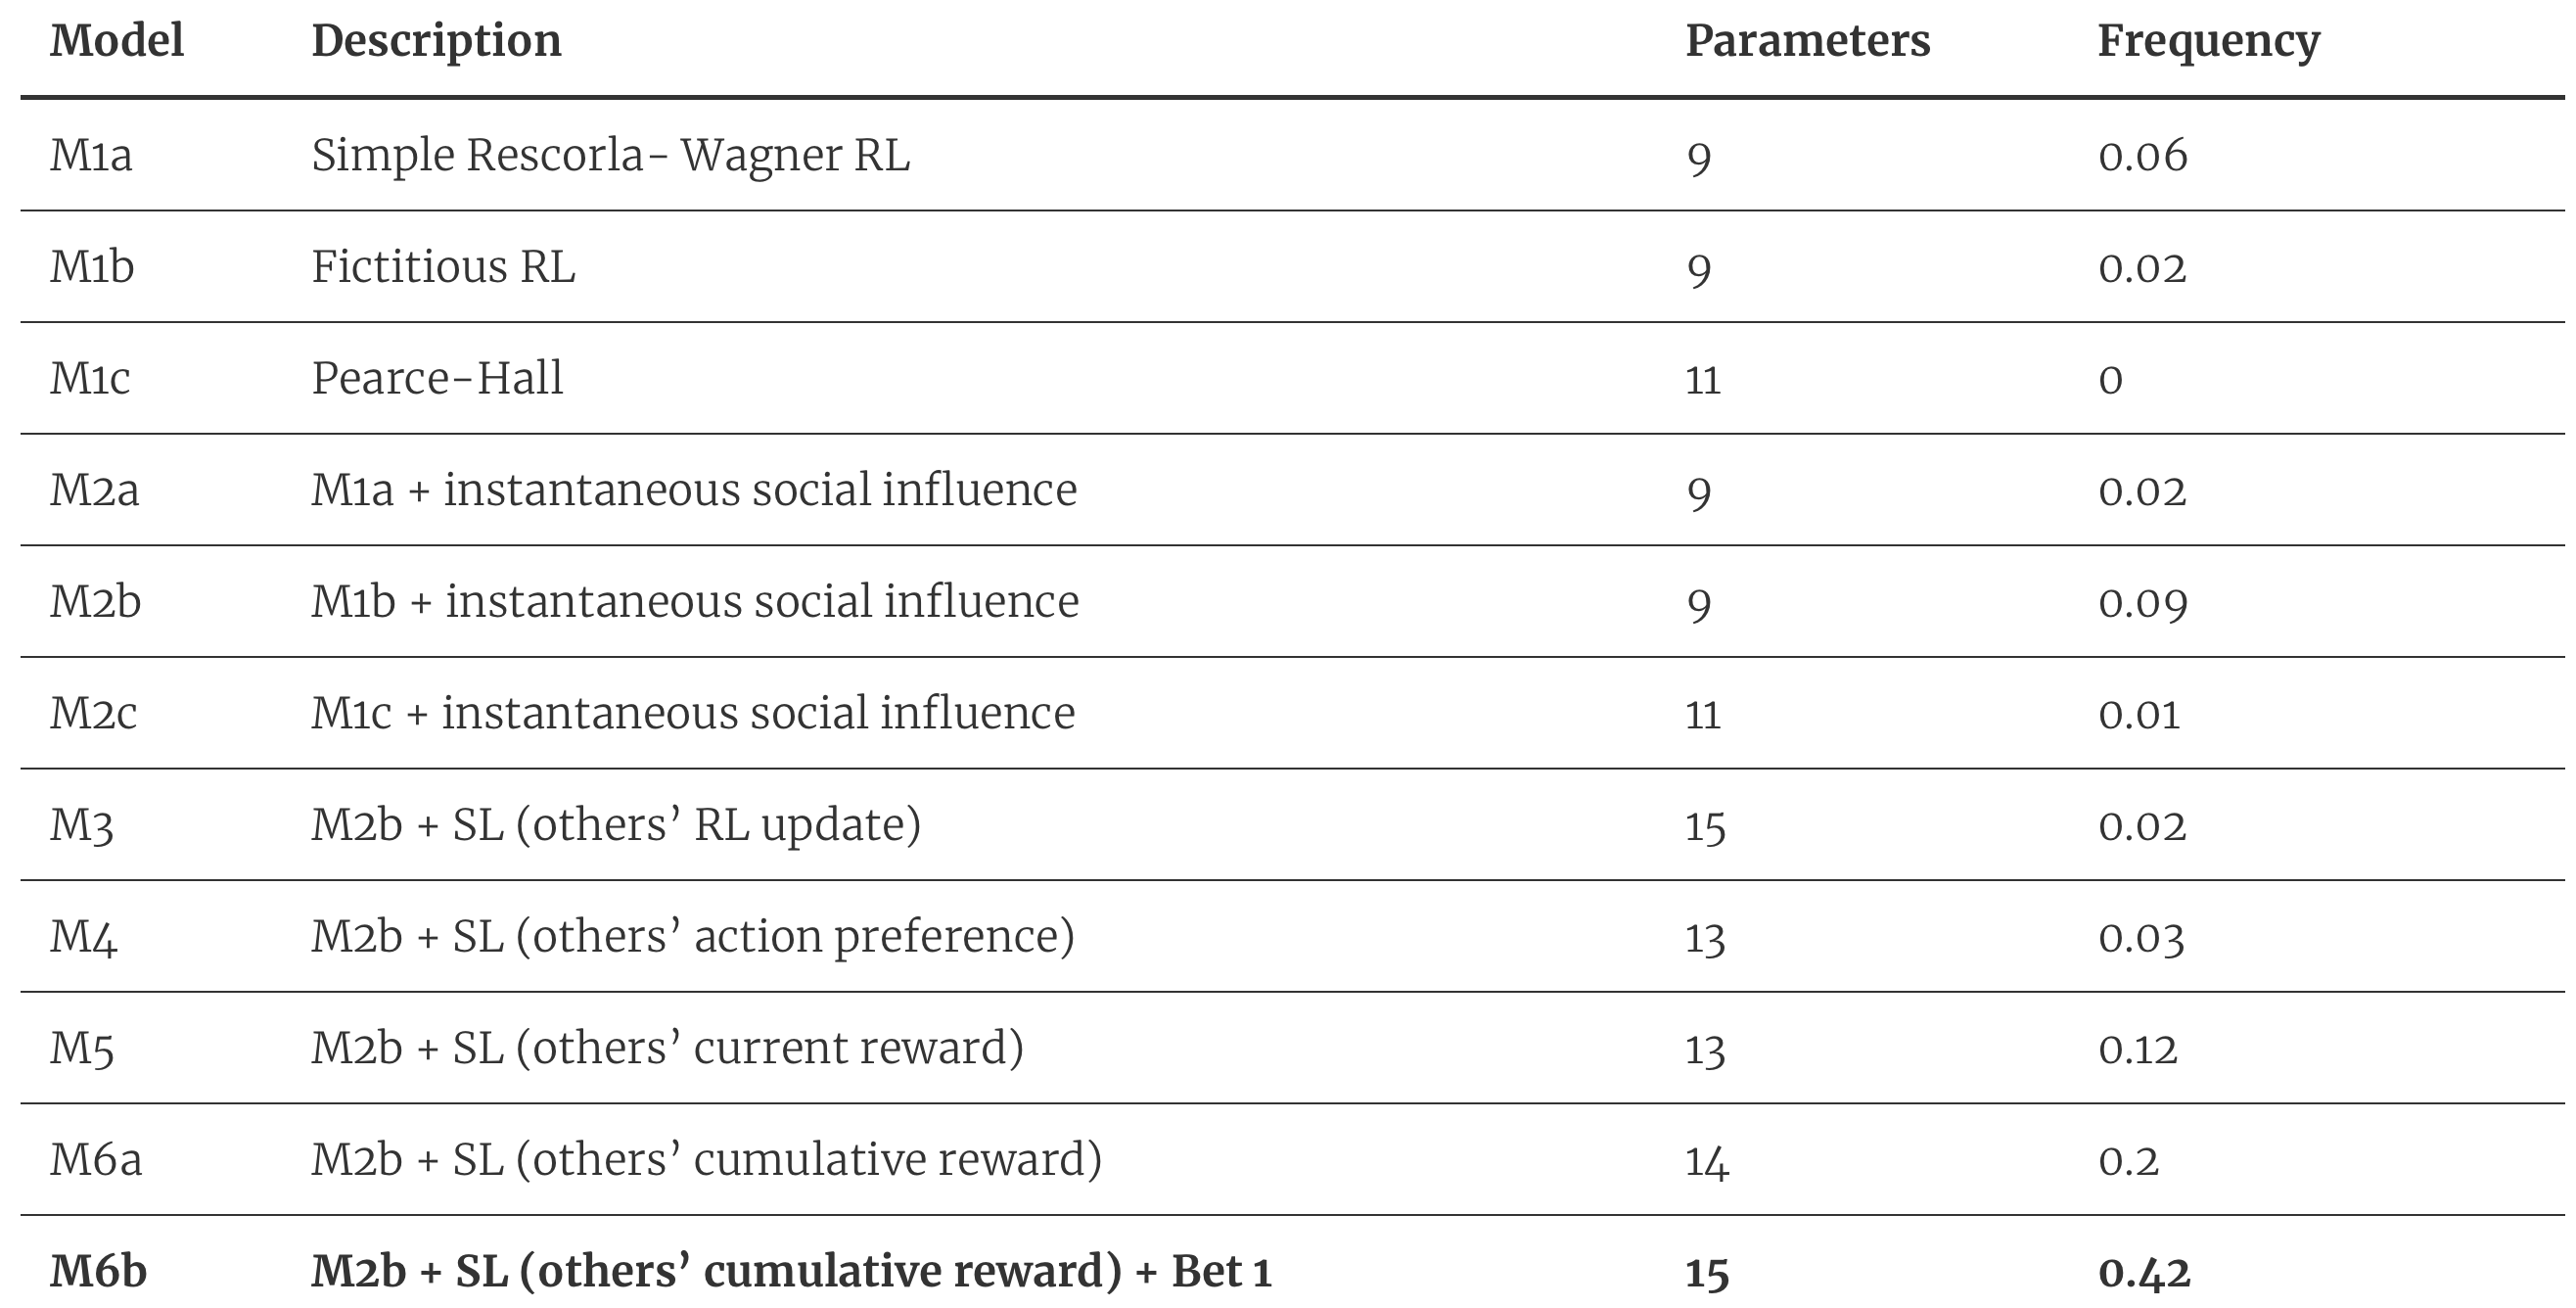
\includegraphics[width=1\linewidth]{figures/models} \caption{{\textbf{Candidate computational models with predicted model frequencies for the entire cohort.} Candidate computational models with predicted model frequencies for the entire cohort. Our candidate models consist of both non-social and social models featuring different parameters. The model with the highest winning frequency (M6b) is highlighted in bold.}}\label{fig:figure-4-models}
\end{figure}



Replicating previous results, we expect for a combined social model (M6b) consisting of a fictitious RL with additional parameters representing instantaneous social influence, bet 1 and other's cumulative reward, to constitute the winning model for the highest proportion of participants. This suggests that most participants jointly integrate value signals computed from direct learning and social learning to guide future decisions. Within the winning model (M6b), parameters reflecting self - Beta(Vself) - and other - Beta(Vother) - should be comparable, both predicting the accuracy of Choice 1. This reflects the integration of self and other-directed information under the combined model (Fig 2.5a). However, we expect for other models to also represent winning models, albeit in fewer participants, demonstrating the heterogeneity in strategy use across our sample (Fig 2.5c). Furthermore, within both M5 and M6a groups, we predict a significantly greater difference between parameters reflecting self - Beta(Vself) - and other - Beta(Vother) - with other-directed information demonstrating a stronger influence.

Across the whole group, we also expect to observe a strong positive relationship between the effect of dissenting social information - Beta(w.Nagainst) - and the susceptibility to social influence, and between the effect of confirming social information - Beta(w.Nwith) - and the extent of bet difference. This suggests that individuals are more likely to change their choice in response to group choice difference, and that confidence increases if a player's choice is also chosen by the group. To determine the transdiagnostic influences upon choice and choice confidence in response to social information, we plan to run separate moderation analyses for each transdiagnostic factor upon the relationships between the effect of dissenting social information - Beta(w.Nagainst) - and the susceptibility to social influence, and the effect between confirming social information - Beta(w.Nwith) - and the extent of bet difference. We subsequently expect for both `Anxious-Depression' and `Social Withdrawal' factors to have a significantly positive moderating effect upon the former and a significantly negative moderating effect upon the latter, reflecting lowered confidence in one's own choices (Fig 2.5b).

Finally, to assess whether the groups within our sample - split by the winning models - differ on the three transdiagnostic symptom dimensions, we will run a linear mixed model predicting the factor scores from an interaction between symptom dimension and group, including a random intercept, and controlling for gender, age, education, and IQ. Reflecting the tendency for those with increased impulsivity and compulsivity to disregard accumulated information, basing decisions on more recent outcomes (Franken et al., 2008; Kim \& Lee, 2011; Robbins et al., 2012; Vaghi et al., 2017), we expect the M5 winning model group (fictitious RL + instantaneous social influence + others' current reward) to feature significantly higher factor scores for `Compulsivity-Impulsivity'. On-the-other-hand, reflecting the ability to integrate historical social information - but not one's own confidence - when making social decisions, we predict for the M6a winning model group (fictitious RL + instantaneous social influence + others' cumulative reward) to feature significantly higher factor scores for `Anxious-Depression' and `Social Withdrawal' (Fig 2.5d).

\begin{figure}
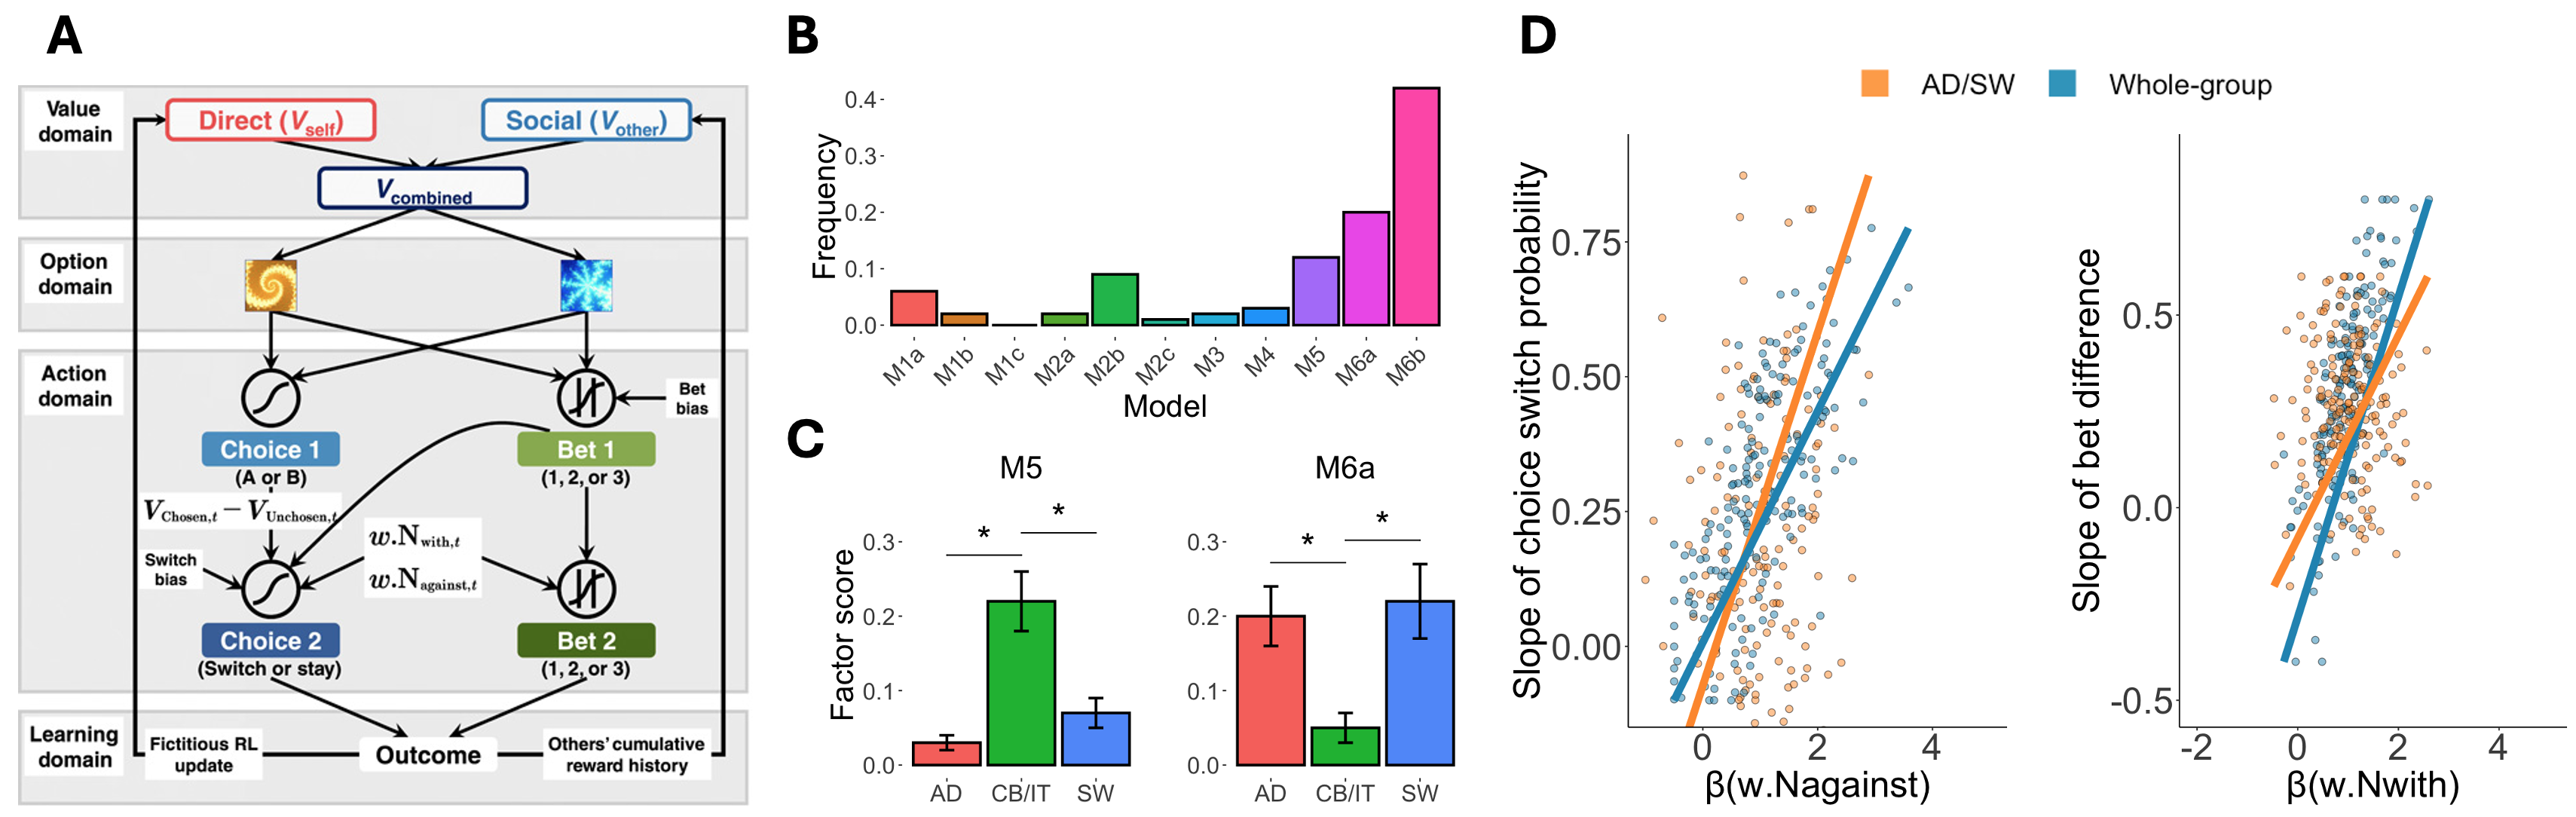
\includegraphics[width=1\linewidth]{figures/predicted_results} \caption{{\textbf{Transdiagnostic factors alter social learning strategies} \textbf{A}) Schematic representation of the winning model (M6b) where participants' initial behaviours were accounted for by value signals updated from direct and social learning and behavioural adjustments ascribed to initial valuation and preference-weighted instantaneous social information (Reproduced from (Zhang \& Gläscher, 2020) with permission). \textbf{B}) Model frequencies across the whole cohort reveal a primary use of the M6b model, but also demonstrate heterogeneity in social learning. \textbf{C}) The winning model groups M5 and M6a feature significantly higher factor scores for `Compulsive Behaviour / Impulsive Thoughts' and both `Anxious-Depression' and `Social Withdrawal' respectively. \textbf{D}) Visual depiction of the influence for both `Anxious-Depression' and `Social Withdrawal' factors upon choice and confidence, where the relationship between the effect of confirming social information - Beta(w.Nwith) - and the extent of bet difference weakens, and the relationship between the effect of dissenting social information - Beta(w.Nagainst) - and the susceptibility to social influence strengthens. Note that this is a visual representation of the moderation analyses, and will not be an actual analysis performed (i.e., a group-level comparison).}}\label{fig:figure-5-results}
\end{figure}



\chapter{Developing a computational psychiatry approach to social anxiety}\label{developing-a-computational-psychiatry-approach-to-social-anxiety}

\chaptermark{}

\noindent  \emph{From this initial study, we aim to subsequently run two follow-up studies focusing on social anxiety, given its prevalence in modern society and relevance to social behaviour. In the first, we will identify the neurocomputational mechanisms underlying altered observational and experiential learning in social anxiety through model-based functional magnetic resonance imaging (fMRI) using the same social influence task. Then, partnering with Alena, a start-up developing digital mental health therapies, we will test the efficacy of smartphone-delivered psychotherapy in reducing behavioural symptoms in social anxiety disorder (SAD).}

\section{Uncovering the neurocomputational mechanisms underlying altered observational and experiential learning in social anxiety}\label{uncovering-the-neurocomputational-mechanisms-underlying-altered-observational-and-experiential-learning-in-social-anxiety}

\subsection{Background}\label{background}

Neuroimaging studies have robustly associated experiential learning with activity of brain regions implicated with reward processing and valuation, including ventromedial prefrontal cortex (vmPFC) representing individuals' own valuation (Bartra et al., 2013) and the ventral striatum (VS)/nucleus accumbens (NAcc) encoding the RPE (O'Doherty et al., 2004) and signalling the rewarding value of potential outcomes (Brosch \& Sander, 2013; Rangel et al., 2008; van der Meer \& Redish, 2010). These regions also play a key role in social decision making (Ruff \& Fehr, 2014), as humans assign intrinsic rewards to social actions (Cushman, 2024; Rilling \& Sanfey, 2011). In social contexts however, an agent might additionally need to integrate information regarding other agent's choices, and emotional states, comprehending the motives behind their actions and weighing the possible outcomes for those involved (Robson et al., 2020; Suzuki \& O'Doherty, 2020). These `socially specific' functions underlying observational learning are computed by the `social brain', a network of brain regions consisting the anterior cingulate cortex (ACC), dorsomedial prefrontal cortex (dmPFC) and temporoparietal junction (TPJ) (Lockwood et al., 2020; Olsson et al., 2020). Ultimately, when making socially relevant decisions, both OL and EL processes are computed within the brain by an integrated hub consisting reward and socially relevant regions that track signals associated with direct experience (vmPFC) and vicarious valuation (ACC) with a combined reward/social prediction error represented in the striatum (NAcc/putamen) (Zhang \& Gläscher, 2020).

The behavioural changes observed in social anxiety and social anxiety disorder (SAD) reflect alterations in brain function, primarily of regions associated with reward sensitivity, valuation, and social processing, with individuals with SAD robustly demonstrating reward network dysfunction in response to both monetary and social rewards (Becker et al., 2017; Cremers et al., 2015; Richey et al., 2014). Resting-state fMRI (rs-fMRI), further highlight changes in amygdala-frontal, parietal-frontal and amygdala-temporal connectivity (Mizzi et al., 2022, 2024), reflecting changes in emotion regulation (Jazaieri et al., 2014), self-referential processing (Whitfield-Gabrieli et al., 2011) and hypervigilance to social threats (Wong \& Rapee, 2016). Changes in social behaviour reinforced through biased learning is similarly mediated by frontoparietal network (FPN) connectivity (Koban et al., 2023), implicated with modulating the top-down regulatory role of self-related content (Dixon \& Gross, 2021). Heightened self-referential processing in SAD is also associated with increased connectivity from the left IPL and PCC to mPFC (Jamieson et al., 2023), (Davey et al., 2016; Davey \& Harrison, 2022), a region implicated with self-representation within social contexts (D'Argembeau, 2013).

\subsection{Study Plan}\label{study-plan}

Socially anxious individuals therefore demonstrate altered activity of prefrontal and striatal regions implicated with observational and experiential learning. We subsequently will use fMRI to uncover the neural components underlying differences in social decision-making driven by OL and EL observed in our initial study, by implementing the same social influence task on two cohorts, with high and low levels of social anxiety (SA) (n = 50 each). Performing perform group-level contrasts (high vs low SA), we expect to observe lowered activity and connectivity of prefrontal-striatal regions associated with monetary and social valuation during the trial outcome and choice preference reveal phases respectively, reflecting a lowered motivation for monetary/social reward. Furthermore, we predict increased activity and connectivity of prefrontal-striatal regions during both choice phases, as socially anxious individuals more strongly engage in self-referential processing when making social decisions. Finally, using model-based fMRI (Gläscher \& O'Doherty, 2010), we expect for the model strategy (M6a) used by the high SA group to be strongly represented with lowered activity of the ventromedial prefrontal cortex (vmPFC) reflecting lowered confidence in the decision process (De Martino et al., 2013).

\section{Digital cognitive behavioural therapy reduces self-referencing in social anxiety disorder}\label{digital-cognitive-behavioural-therapy-reduces-self-referencing-in-social-anxiety-disorder}

\subsection{Background}\label{background-1}

Social anxiety disorder (SAD) is the third most common mental disorder behind substance use disorder and depression (Kessler et al., 2005), and the most common anxiety disorder, with a prevalence of approximately 10\% (Kessler et al., 2005, 2012; Lecrubier et al., 2000). Individuals with SAD, for fear of being negatively judged by others, demonstrate a strong avoidance of social situations, adversely affecting functioning in social roles e.g., increased risk of dropping out of school, reduced workplace productivity, leading to high socioeconomic costs (Keller, 2003; Kessler, 2003). Social anxiety disorder is commonly treated using pharmacological and/or psychological approaches (Ströhle et al., 2018; Szuhany \& Simon, 2022), which take effect in part by altering the processing of social information. Patient responsivity and improvement can therefore be inferred by measuring neural activity in response to specific behavioural paradigms. For example, both forms of treatment dampen the fear response, lowering activity of the amygdala to aversive social stimuli (Goldin et al., 2013; Klumpp et al., 2013), whilst improvements in emotion regulation as a result of cognitive-behavioural therapy (CBT) is associated with increased prefrontal and occipitotemporal activity (Brooks \& Stein, 2022). Symptom reduction in SAD, following CBT, is similarly associated with reduced amygdalar-prefrontal (Yuan et al., 2016) and dorsolateral/dorsomedial prefrontal cortex (dl/dmPFC) activity (Goldin et al., 2021).

A theory-driven approach to psychiatry, generating formal accounts of mental health through computational models (Hauser et al., 2022; Hitchcock et al., 2022; Huys et al., 2016, 2021; Khaleghi et al., 2022), can further determine patient responsivity to treatment by providing an objective measure of the latent cognitive processes shaping brain activity and behaviour (Karvelis et al., 2023). This is particularly relevant for psychotherapy, as a neuro-computational approach can accurately characterise the behaviours and cognitions targeted by CBT (Reiter et al., 2021). Furthermore, as this approach is sensitive to both inter and intra-individual differences (Schaaf et al., 2023), model parameters represent ideal candidates for determining treatment efficacy and can be used in tandem with neuroimaging methods such as fMRI (Sohail \& Zhang, 2024).

\subsection{Study Plan}\label{study-plan-1}

Therefore, we aim in a second fMRI study to uncover the neurocomputational mechanisms underlying patient responsivity to a cognitive-behavioural therapy (CBT) program in SAD. Leveraging the recent trend in digital therapies, we will partner with Alena (Aya Technologies) a start-up specializing in digital mental health who have developed the Alena app, a self-guided CBT programme specifically designed to address social anxiety disorder. The programme is adapted from the Clark and Wells model of social anxiety (Clark \& Wells, 1995) and follows a modular structure, each module targeting a core cognitive component contributing to the maintenance of social anxiety including negative beliefs, self-focused attention, post-event processing/rumination, and avoidance. Importantly, their program leverages a computational psychiatry approach, with gamified behavioural tasks providing objective measures of cognition. Mobile-based therapy further presents a number of advantages over conventional therapies (Gillan \& Rutledge, 2021), including reduced waiting times, dense data phenotyping, increased patient retention, and the development of an individually tailored and manageable program. Furthermore, the absence of a face-to-face social interaction is pertinent to those with SAD as in-person treatments can be aversive. Ultimately, Alena's digital CBT represents a safe, acceptable therapy, showing promising signs of rapid efficacy in the treatment of SAD (Garvert et al., 2023).

In our pre-post study, we aim to recruit forty individuals with a diagnosis of social anxiety disorder. Using fMRI, we will measure brain activity in response to the self-referential encoding task (SRET) (Derry \& Kuiper, 1981), which assesses negative self-referential processing, a major component of the socially anxious phenotype (Talmon et al., 2021) and a behaviour targeted in CBT for SAD (Gregory \& Peters, 2017). Participants after being scanned at baseline, will be randomly allocated to receive CBT-based therapy for social anxiety on the Alena app or to a wait list control group (n = 20 each). Participants randomised to the waitlist control group will subsequently be given access to the app for four weeks after the study is concluded. Comparing brain activity at both timepoints (post vs pre), we expect to observe reduced activity of prefrontal regions implicated in self-referencing and rumination among participants assigned to receive treatment in the app, whilst no changes are expected amongst the control group.

The study will ultimately provide novel scientific evidence for the efficacy underlying a smartphone-based approach in delivering CBT, furthering the development of digital therapies.

\backmatter

\chapter*{References}\label{references}
\addcontentsline{toc}{chapter}{References}

\chaptermark{}

\setlength{\parindent}{0pt}
\setlength{\leftskip}{0em}
\setlength{\parskip}{1em}

Abraham, A., \& Hermann, C. (2015). Biases in probabilistic category learning in relation to social anxiety. Frontiers in Psychology, 6.

Admon, R., \& Pizzagalli, D. A. (2015). Dysfunctional reward processing in depression. Current Opinion in Psychology, 4, 114--118.

Aylward, J., Valton, V., Ahn, W.-Y., Bond, R. L., Dayan, P., Roiser, J. P., \& Robinson, O. J. (2019). Altered learning under uncertainty in unmedicated mood and anxiety disorders. Nature Human Behaviour, 3(10), 1116--1123.

Balietti, S. (2017). nodeGame: Real-time, synchronous, online experiments in the browser. Behavior Research Methods, 49(5), 1696--1715.

Bartra, O., McGuire, J. T., \& Kable, J. W. (2013). The valuation system: A coordinate-based meta-analysis of BOLD fMRI experiments examining neural correlates of subjective value. NeuroImage, 76, 412--427.

Becker, M. P. I., Simon, D., Miltner, W. H. R., \& Straube, T. (2017). Altered activation of the ventral striatum under performance-related observation in social anxiety disorder. Psychological Medicine, 47(14), 2502--2512.

Becker, M. P. I., Voegler, R., Peterburs, J., Hofmann, D., Bellebaum, C., \& Straube, T. (2019). Reward Prediction Error Signaling during Reinforcement Learning in Social Anxiety Disorder is altered by Social Observation (p.~821512). bioRxiv.

Beltzer, M. L., Adams, S., Beling, P. A., \& Teachman, B. A. (2019). Social Anxiety and Dynamic Social Reinforcement Learning in a Volatile Environment. Clinical Psychological Science, 7(6), 1372--1388.

Beltzer, M. L., Daniel, K. E., Daros, A. R., \& Teachman, B. A. (2023). Examining social reinforcement learning in social anxiety. Journal of Behavior Therapy and Experimental Psychiatry, 80, 101810.

Bică, A., Crețu, R. Z., \& Podina, I. R. (2021). Money Versus Social Rank: An Empirical Investigation of Unfairness in Social Anxiety. Cognitive Therapy and Research, 45(4), 642--651.

Bishop, S. J. (2007). Neurocognitive mechanisms of anxiety: An integrative account. Trends in Cognitive Sciences, 11(7), 307--316.

Brooks, S. J., \& Stein, D. J. (2015). A systematic review of the neural bases of psychotherapy for anxiety and related disorders. Dialogues in Clinical Neuroscience, 17(3), 261--279.

Brosch, T., \& Sander, D. (2013). Neurocognitive mechanisms underlying value-based decision-making: From core values to economic value. Frontiers in Human Neuroscience, 7.

Browning, M., Behrens, T. E., Jocham, G., O'Reilly, J. X., \& Bishop, S. J. (2015). Anxious individuals have difficulty learning the causal statistics of aversive environments. Nature Neuroscience, 18(4), 590--596.

Burke, C. J., Tobler, P. N., Baddeley, M., \& Schultz, W. (2010). Neural mechanisms of observational learning. Proceedings of the National Academy of Sciences, 107(32), 14431--14436.

Button, K. S., Browning, M., Munafò, M. R., \& Lewis, G. (2012). Social inference and social anxiety: Evidence of a fear-congruent self-referential learning bias. Journal of Behavior Therapy and Experimental Psychiatry, 43(4), 1082--1087.

Campbell-Meiklejohn, D., Simonsen, A., Frith, C. D., \& Daw, N. D. (2017). Independent Neural Computation of Value from Other People's Confidence. Journal of Neuroscience, 37(3), 673--684.

Carleton, R. N., Collimore, K. C., McCabe, R. E., \& Antony, M. M. (2011). Addressing revisions to the Brief Fear of Negative Evaluation scale: Measuring fear of negative evaluation across anxiety and mood disorders. Journal of Anxiety Disorders, 25(6), 822--828.

Cattell, R. B. (1966). The Scree Test For The Number Of Factors. Multivariate Behavioral Research, 1(2), 245--276.

Chandler, J., Mueller, P., \& Paolacci, G. (2014). Nonnaïveté among Amazon Mechanical Turk workers: Consequences and solutions for behavioral researchers. Behavior Research Methods, 46(1), 112--130.

Charpentier, C. J., Wu, Q., Min, S., Ding, W., Cockburn, J., \& O'Doherty, J. P. (2023). Heterogeneity in strategy use during arbitration between experiential and observational learning. OSF.

Chen, D. L., Schonger, M., \& Wickens, C. (2016). oTree---An open-source platform for laboratory, online, and field experiments. Journal of Behavioral and Experimental Finance, 9, 88--97.

Cremers, H. R., Veer, I. M., Spinhoven, P., Rombouts, S. A. R. B., \& Roelofs, K. (2015). Neural sensitivity to social reward and punishment anticipation in social anxiety disorder. Frontiers in Behavioral Neuroscience, 8.

Cushman, F. (2024). Computational Social Psychology. Annual Review of Psychology, 75(Volume 75, 2024), 625--652.

D'Argembeau, A. (2013). On the Role of the Ventromedial Prefrontal Cortex in Self-Processing: The Valuation Hypothesis. Frontiers in Human Neuroscience, 7.

Davey, C. G., Pujol, J., \& Harrison, B. J. (2016). Mapping the self in the brain's default mode network. NeuroImage, 132, 390--397.

Davey, C. G., \& Harrison, B. J. (2022). The self on its axis: A framework for understanding depression. Translational Psychiatry, 12(1), 1--9.

De Martino, B., Fleming, S. M., Garrett, N., \& Dolan, R. J. (2013). Confidence in value-based choice. Nature Neuroscience, 16(1), 105--110.

Declerck, C. H., Boone, C., \& Emonds, G. (2013). When do people cooperate? The neuroeconomics of prosocial decision making. Brain and Cognition, 81(1), 95--117.

Derry, P. A., \& Kuiper, N. A. (1981). Schematic processing and self-reference in clinical depression. Journal of Abnormal Psychology, 90(4), 286--297.

Dixon, M. L., \& Gross, J. J. (2021). Dynamic network organization of the self: Implications for affective experience. Current Opinion in Behavioral Sciences, 39, 1--9.

Dunne, S., \& O'Doherty, J. P. (2013). Insights from the application of computational neuroimaging to social neuroscience. Current Opinion in Neurobiology, 23(3), 387--392.

Eshel, N., \& Roiser, J. P. (2010). Reward and Punishment Processing in Depression. Biological Psychiatry, 68(2), 118--124.

Fatima, M., \& Ghayas, S. (2017). Relationship between Self-Esteem and Social Anxiety: Role of Social Connectedness as a Mediator (world).

Feczko, E., Miranda-Dominguez, O., Marr, M., Graham, A. M., Nigg, J. T., \& Fair, D. A. (2019). The Heterogeneity Problem: Approaches to Identify Psychiatric Subtypes. Trends in Cognitive Sciences, 23(7), 584--601.

Feng, C., Cao, J., Li, Y., Wu, H., \& Mobbs, D. (2018). The pursuit of social acceptance: Aberrant conformity in social anxiety disorder. Social Cognitive and Affective Neuroscience, 13(8), 809--817.

Foa, E. B., Huppert, J. D., Leiberg, S., Langner, R., Kichic, R., Hajcak, G., \& Salkovskis, P. M. (2002). The Obsessive-Compulsive Inventory: Development and validation of a short version. Psychological Assessment, 14(4), 485--496.

Fox, M. D., \& Greicius, M. (2010). Clinical applications of resting state functional connectivity. Frontiers in Systems Neuroscience, 4.

Franken, I. H. A., van Strien, J. W., Nijs, I., \& Muris, P. (2008). Impulsivity is associated with behavioral decision-making deficits. Psychiatry Research, 158(2), 155--163.

Fried, E. (2017). Moving forward: How depression heterogeneity hinders progress in treatment and research. Expert Review of Neurotherapeutics, 17(5), 423--425.

Garner, D. M., Olmsted, M. P., Bohr, Y., \& Garfinkel, P. E. (1982). The Eating Attitudes Test: Psychometric features and clinical correlates. Psychological Medicine, 12(4), 871--878.

Garvert, M. M., Linke, S., McCloud, T., Meyer, S. S., Sobanska, S., Long, A., Huys, Q. J. M., \& Ahmadi, M. (2023). The Safety, Acceptability and Efficacy of Alena, a Modularized CBT-based Mobile App Intervention for Social Anxiety: A Randomised Controlled Trial (p.~2023.05.30.23288513). medRxiv.

Giamattei, M., Yahosseini, K. S., Gächter, S., \& Molleman, L. (2020). LIONESS Lab: A free web-based platform for conducting interactive experiments online. Journal of the Economic Science Association, 6(1), 95--111.

Gilboa-Schechtman, E., Keshet, H., Livne, T., Berger, U., Zabag, R., Hermesh, H., \& Marom, S. (2017). Explicit and implicit self-evaluations in social anxiety disorder. Journal of Abnormal Psychology, 126(3), 285--290.

Gillan, C. M., Kosinski, M., Whelan, R., Phelps, E. A., \& Daw, N. D. (2016). Characterizing a psychiatric symptom dimension related to deficits in goal-directed control. eLife, 5, e11305.

Gillan, C. M., \& Seow, T. X. F. (2020). Carving Out New Transdiagnostic Dimensions for Research in Mental Health. Biological Psychiatry: Cognitive Neuroscience and Neuroimaging, 5(10), 932--934.

Gillan, C. M., \& Rutledge, R. B. (2021). Smartphones and the Neuroscience of Mental Health. Annual Review of Neuroscience, 44(Volume 44, 2021), 129--151.

Gläscher, J. P., \& O'Doherty, J. P. (2010). Model-based approaches to neuroimaging: Combining reinforcement learning theory with fMRI data. WIREs Cognitive Science, 1(4), 501--510.

Glimcher, P. W. (2013). Neuroeconomics: Decision Making and the Brain. Academic Press.

Goldin, P. R., Ziv, M., Jazaieri, H., Hahn, K., Heimberg, R., \& Gross, J. J. (2013). Impact of Cognitive Behavioral Therapy for Social Anxiety Disorder on the Neural Dynamics of Cognitive Reappraisal of Negative Self-beliefs: Randomized Clinical Trial. JAMA Psychiatry, 70(10), 1048--1056.

Goldin, P. R., Thurston, M., Allende, S., Moodie, C., Dixon, M. L., Heimberg, R. G., \& Gross, J. J. (2021). Evaluation of Cognitive Behavioral Therapy vs Mindfulness Meditation in Brain Changes During Reappraisal and Acceptance Among Patients With Social Anxiety Disorder: A Randomized Clinical Trial. JAMA Psychiatry, 78(10), 1134--1142.

Gorsuch, R. L. (2014). Factor Analysis: Classic Edition (2nd ed.). Routledge.

Gregory, B., \& Peters, L. (2017). Changes in the self during cognitive behavioural therapy for social anxiety disorder: A systematic review. Clinical Psychology Review, 52, 1--18.

Hasler, G. (2012). Can the neuroeconomics revolution revolutionize psychiatry? Neuroscience \& Biobehavioral Reviews, 36(1), 64--78.

Hauser, T. U., Skvortsova, V., Choudhury, M. D., \& Koutsouleris, N. (2022). The promise of a model-based psychiatry: Building computational models of mental ill health. The Lancet Digital Health, 4(11), e816--e828.

Hitchcock, P. F., Fried, E. I., \& Frank, M. J. (2022). Computational Psychiatry Needs Time and Context. Annual Review of Psychology, 73(Volume 73, 2022), 243--270.

Hofheinz, C., Germar, M., Schultze, T., Michalak, J., \& Mojzisch, A. (2017). Are Depressed People More or Less Susceptible to Informational Social Influence? Cognitive Therapy and Research, 41(5), 699--711.

Hopkins, A. K., Gillan, C., Roiser, J., Wise, T., \& Sidarus, N. (2022). Optimising the measurement of anxious-depressive, compulsivity and intrusive thought and social withdrawal transdiagnostic symptom dimensions. OSF.

Hoven, M., Luigjes, J., Denys, D., Rouault, M., \& van Holst, R. J. (2023). How do confidence and self-beliefs relate in psychopathology: A transdiagnostic approach. Nature Mental Health, 1(5), 337--345.

Huys, Q. J. M., Maia, T. V., \& Frank, M. J. (2016). Computational psychiatry as a bridge from neuroscience to clinical applications. Nature Neuroscience, 19(3), 404--413.

Huys, Q. J. M., Browning, M., Paulus, M. P., \& Frank, M. J. (2021). Advances in the computational understanding of mental illness. Neuropsychopharmacology, 46(1), 3--19.

Jamieson, A. J., Harrison, B. J., Delahoy, R., Schmaal, L., Felmingham, K. L., Phillips, L., \& Davey, C. G. (2023). A brain model of altered self-appraisal in social anxiety disorder. Translational Psychiatry, 13(1), 1--9.

Jazaieri, H., Morrison, A. S., Goldin, P. R., \& Gross, J. J. (2014). The Role of Emotion and Emotion Regulation in Social Anxiety Disorder. Current Psychiatry Reports, 17(1), 531.

Joiner, J., Piva, M., Turrin, C., \& Chang, S. W. C. (2017). Social learning through prediction error in the brain. Npj Science of Learning, 2(1), Article 1.

Keller, M. B. (2003). The lifelong course of social anxiety disorder: A clinical perspective. Acta Psychiatrica Scandinavica, 108(s417), 85--94.

Kessler, R. C. (2003). The impairments caused by social phobia in the general population: Implications for intervention. Acta Psychiatrica Scandinavica, 108(s417), 19--27.

Kessler, R. C., Berglund, P., Demler, O., Jin, R., Merikangas, K. R., \& Walters, E. E. (2005). Lifetime Prevalence and Age-of-Onset Distributions of DSM-IV Disorders in the National Comorbidity Survey Replication. Archives of General Psychiatry, 62(6), 593--602.

Kessler, R. C., Petukhova, M., Sampson, N. A., Zaslavsky, A. M., \& Wittchen, H.-U. (2012). Twelve-month and lifetime prevalence and lifetime morbid risk of anxiety and mood disorders in the United States. International Journal of Methods in Psychiatric Research, 21(3), 169--184.

Khaleghi, A., Mohammadi, M. R., Shahi, K., \& Nasrabadi, A. M. (2022). Computational Neuroscience Approach to Psychiatry: A Review on Theory-driven Approaches. Clinical Psychopharmacology and Neuroscience, 20(1), 26--36.

Kim, S., \& Lee, D. (2011). Prefrontal Cortex and Impulsive Decision Making. Biological Psychiatry, 69(12), 1140--1146.
Kishida, K. T., King-Casas, B., \& Montague, P. R. (2010). Neuroeconomic approaches to mental disorders. Neuron, 67(4), 543--554.

Klumpp, H., Fitzgerald, D. A., \& Phan, K. L. (2013). Neural predictors and mechanisms of cognitive behavioral therapy on threat processing in social anxiety disorder. Progress in Neuro-Psychopharmacology and Biological Psychiatry, 45, 83--91.

Koban, L., Schneider, R., Ashar, Y. K., Andrews-Hanna, J. R., Landy, L., Moscovitch, D. A., Wager, T. D., \& Arch, J. J. (2017). Social anxiety is characterized by biased learning about performance and the self. Emotion (Washington, D.C.), 17(8), 1144--1155.

Koban, L., Andrews-Hanna, J. R., Ives, L., Wager, T. D., \& Arch, J. J. (2023). Brain mediators of biased social learning of self-perception in social anxiety disorder. Translational Psychiatry, 13(1), 1--9.

Leary, M. R., Kowalski, R. M., \& Campbell, C. D. (1988). Self-presentational concerns and social anxiety: The role of generalized impression expectancies. Journal of Research in Personality, 22(3), 308--321.

Lecrubier, Y., Wittchen, H. U., Faravelli, C., Bobes, J., Patel, A., \& Knapp, M. (2000). A European perspective on social anxiety disorder. European Psychiatry, 15(1), 5--16.

Lee, D., Seo, H., \& Jung, M. W. (2012). Neural Basis of Reinforcement Learning and Decision Making. Annual Review of Neuroscience, 35(1), 287--308.

Lee, H., \& Chung, D. (2022). Characterization of the Core Determinants of Social Influence From a Computational and Cognitive Perspective. Frontiers in Psychiatry, 13.

Liebowitz, M. R. (1987). Social Phobia.

Lockwood, P. L., Apps, M. A. J., \& Chang, S. W. C. (2020). Is There a `Social' Brain? Implementations and Algorithms. Trends in Cognitive Sciences, 24(10), 802--813.

Lockwood, P. L., \& Klein-Flügge, M. C. (2021). Computational modelling of social cognition and behaviour---A reinforcement learning primer. Social Cognitive and Affective Neuroscience, 16(8), 761--771.

Loewenstein, G., Rick, S., \& Cohen, J. D. (2008). Neuroeconomics. Annual Review of Psychology, 59(Volume 59, 2008), 647--672.

Maia, T. V., \& Frank, M. J. (2011). From reinforcement learning models to psychiatric and neurological disorders. Nature Neuroscience, 14(2), 154--162.

Marin, R. S., Biedrzycki, R. C., \& Firinciogullari, S. (1991). Reliability and validity of the apathy evaluation scale. Psychiatry Research, 38(2), 143--162.

Mizzi, S., Pedersen, M., Lorenzetti, V., Heinrichs, M., \& Labuschagne, I. (2022). Resting-state neuroimaging in social anxiety disorder: A systematic review. Molecular Psychiatry, 27(1), 164--179.

Mizzi, S., Pedersen, M., Rossell, S. L., Rendell, P., Terrett, G., Heinrichs, M., \& Labuschagne, I. (2024). Resting-state amygdala subregion and precuneus connectivity provide evidence for a dimensional approach to studying social anxiety disorder. Translational Psychiatry, 14(1), 1--10.

O'Doherty, J., Dayan, P., Schultz, J., Deichmann, R., Friston, K., \& Dolan, R. J. (2004). Dissociable Roles of Ventral and Dorsal Striatum in Instrumental Conditioning. Science, 304(5669), 452--454.

O'Doherty, J. P., Cockburn, J., \& Pauli, W. M. (2017). Learning, Reward, and Decision Making. Annual Review of Psychology, 68(1), 73--100.

O'Doherty, J. P., Lee, S. W., Tadayonnejad, R., Cockburn, J., Iigaya, K., \& Charpentier, C. J. (2021). Why and how the brain weights contributions from a mixture of experts. Neuroscience \& Biobehavioral Reviews, 123, 14--23.

Olsson, A., Knapska, E., \& Lindström, B. (2020). The neural and computational systems of social learning. Nature Reviews Neuroscience, 21(4), Article 4.

Pärnamets, P., \& Olsson, A. (2020). Integration of social cues and individual experiences during instrumental avoidance learning. PLOS Computational Biology, 16(9), e1008163.

Patton, J. H., Stanford, M. S., \& Barratt, E. S. (1995). Factor structure of the barratt impulsiveness scale. Journal of Clinical Psychology, 51(6), 768--774.

Peterburs, J., Albrecht, C., \& Bellebaum, C. (2022). The impact of social anxiety on feedback-based go and nogo learning. Psychological Research, 86(1), 110--124.

Pike, A. C., \& Robinson, O. J. (2022). Reinforcement Learning in Patients With Mood and Anxiety Disorders vs Control Individuals: A Systematic Review and Meta-analysis. JAMA Psychiatry, 79(4), 313--322.

Piray, P., Ly, V., Roelofs, K., Cools, R., \& Toni, I. (2019). Emotionally Aversive Cues Suppress Neural Systems Underlying Optimal Learning in Socially Anxious Individuals. Journal of Neuroscience, 39(8), 1445--1456.

Rangel, A., Camerer, C., \& Montague, P. R. (2008). A framework for studying the neurobiology of value-based decision making. Nature Reviews Neuroscience, 9(7), 545--556.

Rangel, A. (2009). Chapter 28---The Computation and Comparison of Value in Goal-directed Choice. In P. W. Glimcher, C. F. Camerer, E. Fehr, \& R. A. Poldrack (Eds.), Neuroeconomics (pp.~425--440). Academic Press.

Rangel, A., \& Hare, T. (2010). Neural computations associated with goal-directed choice. Current Opinion in Neurobiology, 20(2), 262--270.

Read Montague, P. (2018). Chapter 11---Computational Phenotypes Revealed by Interactive Economic Games. In A. Anticevic \& J. D. Murray (Eds.), Computational Psychiatry (pp.~273--292). Academic Press.

Reiter, A. M., Atiya, N. A., Berwian, I. M., \& Huys, Q. J. (2021). Neuro-cognitive processes as mediators of psychological treatment effects. Current Opinion in Behavioral Sciences, 38, 103--109.

Richey, J. A., Rittenberg, A., Hughes, L., Damiano, C. R., Sabatino, A., Miller, S., Hanna, E., Bodfish, J. W., \& Dichter, G. S. (2014). Common and distinct neural features of social and non-social reward processing in autism and social anxiety disorder. Social Cognitive and Affective Neuroscience, 9(3), 367--377.

Rilling, J. K., \& Sanfey, A. G. (2011). The Neuroscience of Social Decision-Making. Annual Review of Psychology, 62(Volume 62, 2011), 23--48.

Robbins, T. W., Gillan, C. M., Smith, D. G., Wit, S. de, \& Ersche, K. D. (2012). Neurocognitive endophenotypes of impulsivity and compulsivity: Towards dimensional psychiatry. Trends in Cognitive Sciences, 16(1), 81--91.

Robson, S. E., Repetto, L., Gountouna, V.-E., \& Nicodemus, K. K. (2020). A review of neuroeconomic gameplay in psychiatric disorders. Molecular Psychiatry, 25(1), 67--81.

Rouault, M., Seow, T., Gillan, C. M., \& Fleming, S. M. (2018). Psychiatric Symptom Dimensions Are Associated With Dissociable Shifts in Metacognition but Not Task Performance. Biological Psychiatry, 84(6), 443--451.

Ruff, C. C., \& Fehr, E. (2014). The neurobiology of rewards and values in social decision making. Nature Reviews Neuroscience, 15(8), 549--562.

Schaaf, J. V., Weidinger, L., Molleman, L., \& van den Bos, W. (2023). Test--retest reliability of reinforcement learning parameters. Behavior Research Methods.

Seema, G. B., \& Kumar, G. V. (2017). Self-Esteem and Social Anxiety in Adolescent Students. Journal of Psychosocial Research, 12(2), 247--254.

Seow, T. X. F., \& Gillan, C. M. (2020). Transdiagnostic Phenotyping Reveals a Host of Metacognitive Deficits Implicated in Compulsivity. Scientific Reports, 10(1), 2883.

Serra, D. (2021). Decision-making: From neuroscience to neuroeconomics---an overview. Theory and Decision, 91(1), 1--80.
Spielberger, C. D. (1970). Manual for the State-Trait Anxiety Inventory (Self-evaluation Questionnaire). (No Title).

Sohail, A., \& Zhang, L. (2024). Informing the treatment of social anxiety disorder with computational and neuroimaging data. Psychoradiology, kkae010.

Spokas, M. E., \& Cardaciotto, L. (2014). Heterogeneity Within Social Anxiety Disorder. In The Wiley Blackwell Handbook of Social Anxiety Disorder (pp.~247--267). John Wiley \& Sons, Ltd.

Ströhle, A., Gensichen, J., \& Domschke, K. (2018). The Diagnosis and Treatment of Anxiety Disorders. Deutsches Arzteblatt International, 155(37), 611--620.

Sutton, R. S., \& Barto, A. G. (2018). Reinforcement Learning, second edition: An Introduction. MIT Press.

Suzuki, S., \& O'Doherty, J. P. (2020). Breaking human social decision making into multiple components and then putting them together again. Cortex, 127, 221--230.

Szuhany, K. L., \& Simon, N. M. (2022). Anxiety Disorders: A Review. JAMA, 328(24), 2431--2445.

Talmon, A., Dixon, M. L., Goldin, P. R., Heimberg, R. G., \& Gross, J. J. (2021). Neurocognitive Heterogeneity in Social Anxiety Disorder: The Role of Self-Referential Processing and Childhood Maltreatment. Clinical Psychological Science, 9(6), 1045--1058.

Tomlin, D., Nedic, A., Prentice, D. A., Holmes, P., \& Cohen, J. D. (2013). The Neural Substrates of Social Influence on Decision Making. PLOS ONE, 8(1), e52630.

Trudel, N., Lockwood, P. L., Rushworth, M. F., \& Wittmann, M. K. (2023). Neural activity tracking identity and confidence in social information. eLife, 12, e71315.

Vaghi, M. M., Luyckx, F., Sule, A., Fineberg, N. A., Robbins, T. W., \& De Martino, B. (2017). Compulsivity Reveals a Novel Dissociation between Action and Confidence. Neuron, 96(2), 348-354.e4.

Van Der Meer, M. A. A., \& Redish, A. D. (2010). Expectancies in decision making, reinforcement learning, and ventral striatum. Frontiers in Neuroscience, 3.

Voegler, R., Peterburs, J., Bellebaum, C., \& Straube, T. (2019). Modulation of feedback processing by social context in social anxiety disorder (SAD)--an event-related potentials (ERPs) study. Scientific Reports, 9(1), 4795.

Wechsler, D. (2019). Wechsler Adult Intelligence Scale---Third Edition {[}dataset{]}.

Wells, A., Clark, D. M., Salkovskis, P., Ludgate, J., Hackmann, A., \& Gelder, M. (1995). Social phobia: The role of in-situation safety behaviors in maintaining anxiety and negative beliefs. Behavior Therapy, 26(1), 153--161.

Whitfield-Gabrieli, S., Moran, J. M., Nieto-Castañón, A., Triantafyllou, C., Saxe, R., \& Gabrieli, J. D. E. (2011). Associations and dissociations between default and self-reference networks in the human brain. NeuroImage, 55(1), 225--232.

Wong, Q. J. J., \& Rapee, R. M. (2016). The aetiology and maintenance of social anxiety disorder: A synthesis of complementary theoretical models and formulation of a new integrated model. Journal of Affective Disorders, 203, 84--100.

Zabag, R., Gilboa-Schechtman, E., \& Levy-Gigi, E. (2022). Reacting to changing environment: Updating patterns in social anxiety. Behaviour Research and Therapy, 157, 104159.

Zabag, R., Azoulay, R., Rinck, M., Becker, E., Levy-Gigi, E., \& Gilboa-Schechtman, E. (2023). You never get a chance to undo a negative first impression: Social anxiety is associated with impaired positive updating of social information. Personality and Individual Differences, 203, 111993.

Zhang, L., \& Gläscher, J. (2020). A brain network supporting social influences in human decision-making. Science Advances, 6(34), eabb4159.

Zung, W. W. K. (1965). A Self-Rating Depression Scale. Archives of General Psychiatry, 12(1), 63--70.

\backmatter

\end{document}
